\chapter{Introduction}
Particle Physics or sometimes called High Energy Physics$:$ is the field of physics that pursues the ultimate structure of matter, this possible in two ways, one is to look for elementary particles, the ultimate constituents of matter at their smallest scale and the other is to clarify what interactions are acting among them $(forces)$ to construct matter as we see it.
 
There are four forces in nature, gravity, electromagnetism, weak nuclear force and strong nuclear force. In this essay our work will be on the strong nuclear force. 

\section{Strong Force}
The gauge bosons that mediate this interactions are eight gauge bosons called gluons, which come from the gauge group $SU(3)$ which has eight generators, gluons mediate the interaction between quarks.

Gluon is massless spin $1$ particle, carrying charge called colour charges, glouns look like photons but photons do not carry electric charge, because of this glouns can interact among themselves unlike photons.
Normally the range of the force can be calculated by a simple argument of the uncertainty, but this not the case for the strong force, the strong force is more complicated and involves a concept known as confinement.

The colour charge has strange property that it exerts a constant force that binds colour carrying particles together, this can be visualized using the analogy of a rubber band, the stronger you pull on the rubber band the tighter it feels. If you do not pull on it at all, it hang loose. The same thing happens for the particles,  that   means at a very short distance, the force is relaxed and the particles behave as a free particles, as the distance between them increases the force act like a rubber band, the force get them back in stronger pulling and when the rubber band is stretched beyond its limits then it will cut into many pieces producing more hadrons.  This phenomenon is known as the colour confinement. In other words those particle tend not be separated by a macroscopic distance.  
This limits the range of strong force, which is believed to be on order of $10^{-15}m$, the dimension of a nuclear particle.

The theory which describes this force is called $Quantum$ $Chromodynamics$.
\section{Quarks}
Quarks and leptons are the building blocks which build up matter. In the present there are six "flavours" of quarks, these are up, down charm strange, top and bottom, and can written as
        \begin{equation*} \left( \begin{array}{c}          
           \text{up}\\
           \text{down}\\
         \end{array}
         \right);  \hspace{1cm}    
     \left (\begin{array}{c}
              \text{charm}\\
              \text{strange}\\
               \end{array}
                 \right)  ;  \hspace{1cm} 
               \left( \begin{array}{c}
                       \text{top}\\
                       \text{bottom}\\
                      \end{array}
                     \right) \end{equation*}  
                         
Quarks can successfully a count for all known mesons and baryon, where mesons are consist of quark and anti quark and baryons are consist of three quarks or three anti quarks. 

Quarks carry colour quantum number: red, green or blue, since all hadrons are colour charge neutral, they must have white charge. 

Unlike other elementary particles quarks carry fractional charge and posses new quantum number. The next table summarize some properties of quarks. Each quark flavour is associated with an own quantum number, which is conserved in strong and electromagnetic interactions but not in weak interaction.
These are: 

\noindent -Strangeness: $S=-1$ for s-quark. 

-Charm: $C=+1$ for c-quark. 

-Beauty: $\tilde{B}=-1$ for b-quark 
-t-quark has life time too short to form hadrons 

-up and down quarks have nameless flavor quantum numbers.\citep{particle}

\begin{table}
\begin{center} 
 \begin{tabular}{|c|c|c|c|} \hline 
  Name (flavour) & symbol & charge(in units of e) & mass  \\ \hline 
  $\text{Up}$ & $\text{U}$ &$ +\frac{3}{2}$ & $1.7-3.1 \frac{Mev}{c^2}$\\\hline
  $\text{Down}$&$\text{d}$&$-\frac{1}{3}$& $4.1-5.7\frac{Mev}{c^2}$\\\hline
  $\text{charm}$&$\text{d}$&$+\frac{1}{3}$&$1.18-1.34\frac{Gev}{c^2}$\\\hline
  $\text{strange}$&$\text{d}$&$-\frac{1}{3}$&$80-130\frac{Mev}{c^2}$\\\hline
  $\text{top}$&$\text{d}$&$+\frac{1}{3}$&$172.3-173.5\frac{Gev}{c^2}$\\\hline
  $\text{bottom}$&$\text{d}$&$-\frac{1}{3}$&$4.13-4.37\frac{Gev}{c^2}$\\\hline
 \end{tabular}
 \caption{properties of Quarks}
\end{center}
\end{table}

\section{Large Hadron Collider}

Hadron colliders are devices made to explore the world of particle physics, they work as theories testers and also as a discovery machines, an example of these hadron colliders is the LHC in CERN. In the Large hadron collider two beams of hadrons(protons) are being accelerated to a high kinetic energy and then collided with each other. It has started operation in 2009 and in 2013 the Higgs particle has been discovered in LHC. Most of the interesting physics at LHC involves investigating the results of these interactions(collisions), as a result of this collision stable partons are formed, partons consists of quarks and qluons. Because of the complex nature of the event at the hadrons colliders, the description of the final state involves a multi-particle calculations. The accurate prediction of the final state in hadron colliders is still one the hardest problems, this problem roots to the non-abelian nature of QCD, which leads to a colour confinement at a long distances. The two main problems are the description of the hadron formation and the evolution of QCD final states from short to long distances. Those problems can be tackled to a good approximation by Monte-Carlo event generators. 

\section{The Parton Shower}
In general parton showers are approximations of the higher order real emission corrections to the hard scattering. The word hard here means, the process involves a transfer of large momentum, either a violent scatter or creation of large mass. They locally conserve flavour and four momentum, and also they are consistent, which means, the particle either splits into two or not. 
Since the parton showers are simulate of the branching and splitting processes, the quality of their predictions depend on precise is the implementation, for example one can ensure the colour coherence through selecting an evolution variable representing the angular ordering, although, this in not the only choice to ensure the colour coherence \citep{introduction}. In the following we will at a simple implementation of a parton shower in python.   
\section{Hadronization}  

To reflect the colour neutrality of the particles in our model the partons will be transformed into a stable hadrons which are colour neutral, this process is called hadronization. The first implemented model and also follows Monte-Carlo event generators was Feynman-Field Model, which gives an idea of the formation of the mesons through iteratively from a single quark. However, this model is not collinear safe, which means the model can mix the short and long distance physics. Now a days two models are common, the string model and clustering model\citep{introduction}. 
     
      
\section{Monte Carlo Method}
Monte Carlo method is set of mathematical tools that first used by scientist to generate game chance that its behaviour can be used to study interesting phenomena. In our context the definition of Monte Carlo method would be, that in which the usage of random numbers is deliberate in a calculation that involves a sequence of states whose  evolution can be considered random\citep{introduction}. 
\subsection{Pseudo-random numbers}
In a computer these are generated using a deterministic algorithm that generates a set of numbers that exhibits statistical randomness, those numbers are called pseudo-random.[the book] 

The main properties of a good random generator are:

\begin{itemize}
\item[•]\textbf{Long period}: the pseudo-random generators have a finite range after which they begin to repeat themselves, for a good random generator this range should much longer than the amount of numbers that are needed for the calculation. 

\item[•]\textbf{Randomness}: The numbers should follow the uniform distribution and also should be independent of each other. 

\item[•]\textbf{Repeatability}: The same initial values should give the same sequence of a random numbers, this important for testing because one might need to repeat the calculation or in the coding terms debugging.

\item[•]\textbf{Portability}: One should be able to generate the same sequence in different machines. 

\item[•]\textbf{Fast}: the generation of the pseudo-random numbers should not be time consuming\citep{Weinzierl}.    
\end{itemize}



\subsection{Samples with different PDFs}
Generating samples of different probability distribution function(pdf) is essential since we are simulating various variables that have different numerical behaviour. For example if our pseudo-random numbers are uniformly distributed in the interval [0,1] and a sequence of specified distribution is needed. I will mention two methods, which are used in this essay. 

\subsection{The acceptance-rejection method}
The acceptance-rejection method was developed by von Neumann. Assume we have a sample x which is uniformly distributed and the pdf is denoted by f(x), and the unknown pdf is denoted by p(x), we assume that we can enclose p(x) inside a shape that is f(x).

In simple words, one first generates x according to the uniform distribution and then calculates p(x) and f(x), then generates another number which is also uniformly distributed, and checks  $y \times f(x) \leq p(x)$. If this the case then accept x, if not reject x and start again. Example of this method is calculation of pi, assume we have a box of side length D and a circle of diameter D inside that box, now the probability that a point in the box and is also in the circle is approximately the area of the circle over the area of the box, which is $\pi$ over 4 here, hence, from this we can approximate the value of $\pi$. The histograms in Figure 1 exhibits this calculation and also the error in the calculation\citep{Weinzierl}. 

\begin{figure}
    \centering
    \begin{subfigure}[b]{0.45\textwidth}
        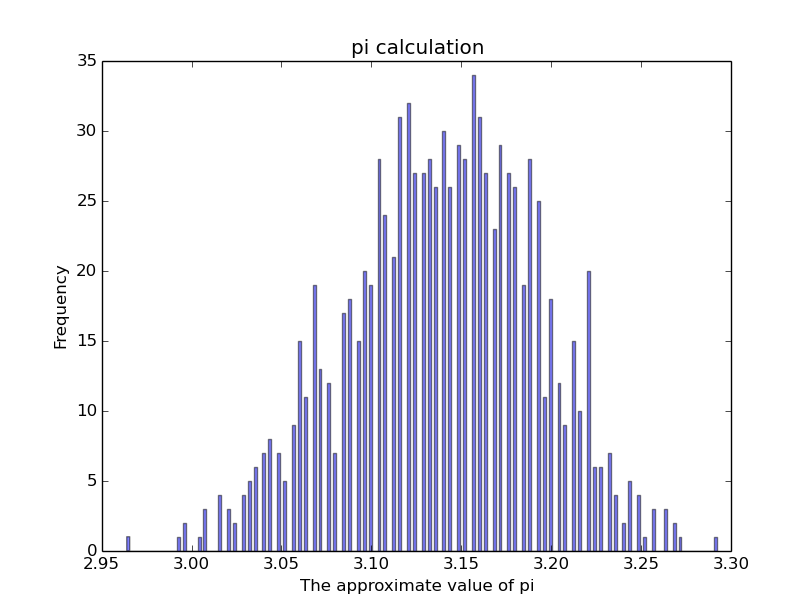
\includegraphics[scale=.45]{images/pi_value.png} 
        \caption{pi value}
        \label{fig:gull}
    \end{subfigure}
    ~ %add desired spacing between images, e. g. ~, \quad, \qquad, \hfill etc. 
      %(or a blank line to force the subfigure onto a new line)
    \begin{subfigure}[b]{0.45\textwidth}
        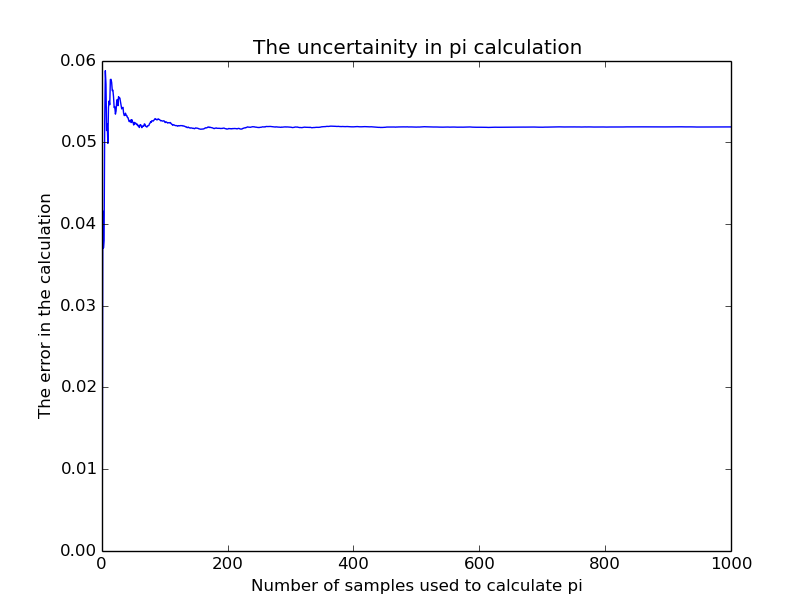
\includegraphics[width=\textwidth]{images/uncertainity_pi.png}
        \caption{The uncertainty}
        \label{fig:tiger}
    \end{subfigure}
    \label{Fig:1}
\caption{}
\end{figure}

\subsection{The inverse transform method} 

Let x be a random with pdf $p(x)$ that takes values in the interval [0,1] and let y be a random variable that is uniformly distributed in the interval [0,1]. We set
\begin{equation}
x = p^-1(y)
\end{equation}
One application of this method is the importance sampling, in which certain values are preferred\citep{Weinzierl}. Example of this is generating an angle theta in the interval $[0,\pi/2]$ that is inversely distributed, where the small angles are desired. The histograms in figure 2 demonstrate this and the error in the calculation.    

\begin{figure}
    \centering
    \begin{subfigure}[b]{0.45\textwidth}
        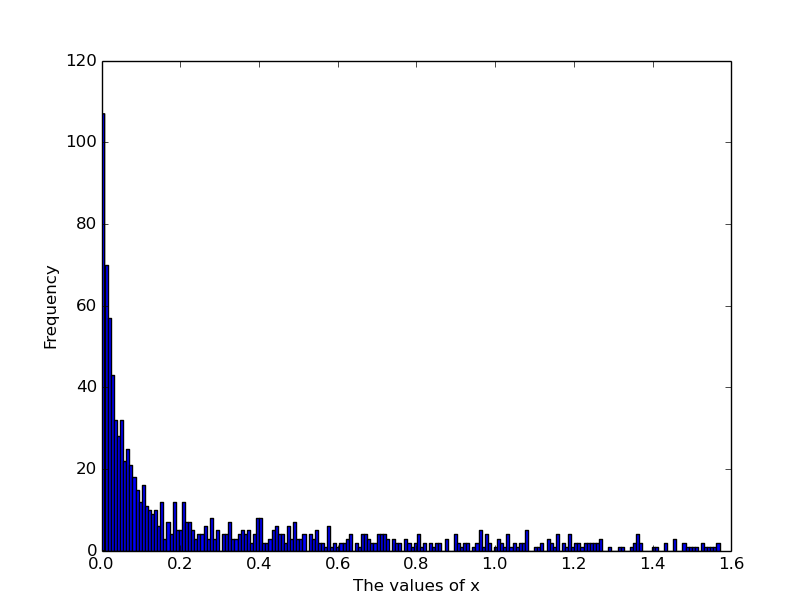
\includegraphics[width=\textwidth]{images/inverse_method.png}
        \caption{Theta values}
        \label{fig2}
    \end{subfigure}
    ~ %add desired spacing between images, e. g. ~, \quad, \qquad, \hfill etc. 
      %(or a blank line to force the subfigure onto a new line)
    \begin{subfigure}[b]{0.4\textwidth}
        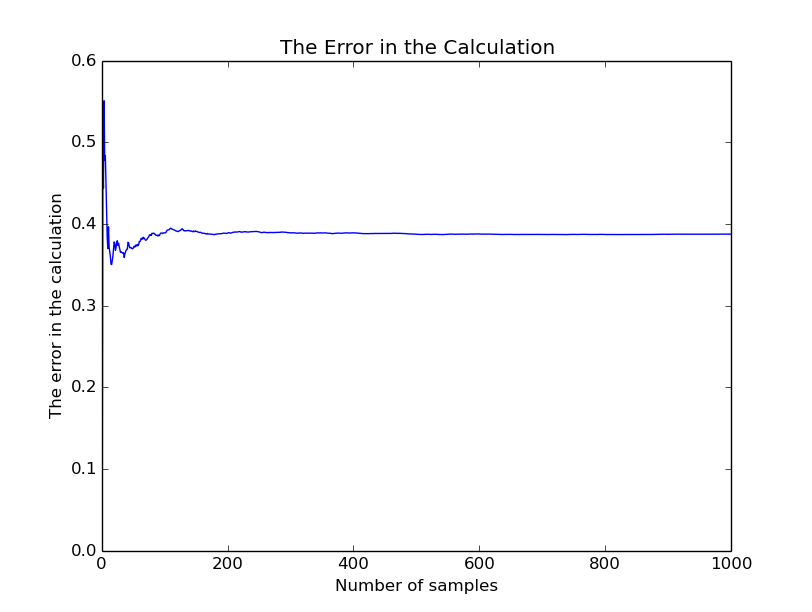
\includegraphics[width=\textwidth]{images/uncertainity_.png}
        \caption{The uncertainty}
        \label{fig2}
    \end{subfigure}
    \label{Fig:1}
\caption{}
\end{figure}

\subsection{The module random in python}

The samples above were generated using $python$ module random, here are few words about this module.
 
This module implements pseudo-random number generators for various distributions.

For integers, there is uniform selection from a range. For sequences, there is uniform selection of a random element, a function to generate a random permutation of a list in-place, and a function for random sampling without replacement.

On the real line, there are functions to compute uniform, normal (Gaussian), lognormal, negative exponential, gamma, and beta distributions. For generating distributions of angles, the von Mises distribution is available.

Almost all module functions depend on the basic function random(), which generates a random float uniformly in the semi-open range $[0.0, 1.0)$. Python uses the Mersenne Twister as the core generator. It produces 53-bit precision floats and has a period of $2**19937-1$. The underlying implementation in C is both fast and threadsafe. The Mersenne Twister is one of the most extensively tested random number generators in existence.
\section{Parton Shower Simulation}
The following is a simple simulation in python for a splitting of a single quark, the simulation accounts for the four momentum conservation of the soft particles.    
\subsection{Physical description}
\noindent As a result of a hadrons collision, quarks will fly away. Since they are charged particles(colour charge), the moving quarks will radiate. The quark will lose part of its energy emitting a gluon. If at the beginning, the quark had energy $E_i$ and radiates energy $E_{rad}$, then the qluon takes $\frac{E_{rad}}{E_i}$ of the particle's initial energy. It is radiated at an angle of $\theta$ to the quark initial direction. The quark will fly on radiating another gluon and so on until it becomes stable(the hadronization starts). The radiated gluons will decay into two quarks, which will later radiates gluons,  which will radiate gluons again and so on. The result is a shower of partons decaying into two partons. 
\begin{figure}[hbtp]
%\caption{}
\centering
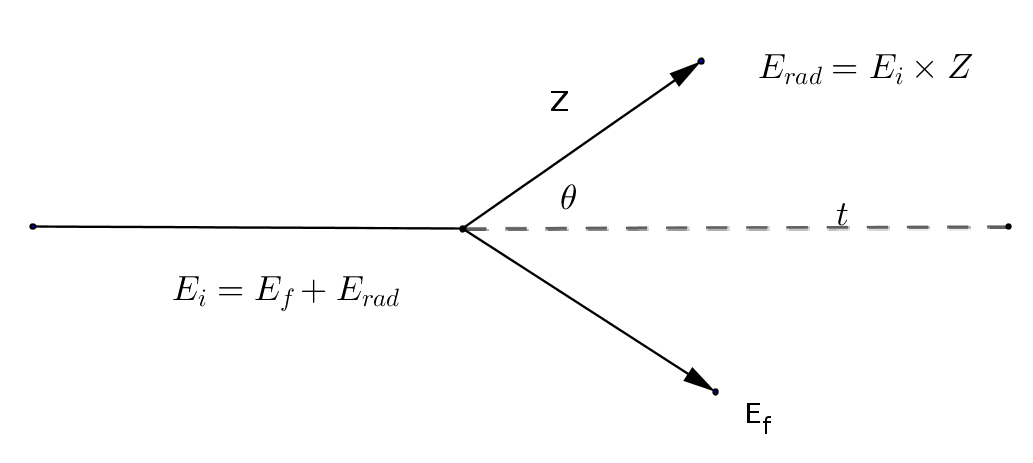
\includegraphics[scale=.15]{images/tt.png}
\end{figure}


Now we begin with 4- momentum vector \begin{equation}
P^{\mu} = \begin{pmatrix}
E/c& \\p_x&\\ p_y &\\ p_z 
\end{pmatrix}
; 
P_{\mu} = \begin{pmatrix}
E/c& \\-p_x&\\-p_y &\\ -p_z 
\end{pmatrix}
\end{equation}   And the inner product is given by \begin{equation}
P^{\mu} P_{\mu} = P^{\mu} \eta_{\mu \nu} P_{\nu} =  (m_0 c)^2 
\end{equation} \begin{equation} P^{\mu} P_{\mu} = \left(\frac{E}{c}\right)^2 - (p_x^2 + p_y^2 + p_z^2) = (m_0 c)^2 \end{equation} Now considering the natural units $c =1$ this can be written as \begin{equation}\label{4} m_0^2 = E^2 - \Vert p \Vert \end{equation} Which is lorentz invariant quantity i.e does not depend on the frame. In our case the quarks in (LHC), the mass of the quark $\sim$ 1 Mev and the energy of the hadrons is $\sim$ 1 Tev, hence, we can assume that the mass of the quark(\ref{4}) is $0$.

From the conservation of energy and momentum, 

\begin{equation}
P_{i}^{\mu} = P_f^{\mu}.
\end{equation} 
We assume that the intial patricle is moving in x -direction, we can write the initial 4-momentum as $P_i^{\mu} = (E,E,0,0)$, afterwards the particle will split. Therefore, the final momentum is given by $P_{rad} + P_{part}$, part here refers to the particle which has lost part of its energy, so $P_{rad} = (E_{rad},\  cos\theta \cdot E_{rad},\  sin\theta \cdot E_{rad},\ 0)$. From this, and since the particle is rotated with $\theta$ we can find the direction of the particle(part) with help of the rotation matrix \begin{equation} R = 
\begin{pmatrix}
\cos\theta & - sin\theta\\
\sin\theta & \cos\theta
\end{pmatrix}
\end{equation} The direction of the particle of the fraction enregy can be found using the following equation  \begin{equation}
P_{part} = P_{i} - P_{rad} .
\end{equation}    
In a three dimensional world, we have two rotation angles, the angular angle and the azimuthal angle. Given a unit vector $u =(u_x, u_y, u_z) $, where $u_x^2 + u_y^2 + u_z^2 = 1$,the matrix for rotating this particle by angle $\theta$ about an axis in the direction of $u$ is   
\begin{equation} 
\begin{pmatrix}
\cos\theta + u^2_x(1-\cos\theta) & u_x u_y (1-\cos\theta) - u_z \sin\theta& u_x u_z(1-\cos\theta)+ u_y \sin\theta\\

u_y u_x (1 - \cos\theta) + u_z \sin\theta & \cos\theta + u_y^2 (1 - \cos\theta) & u_y u_z (1 - \cos\theta) - u_x \sin\theta \\

u_z u_x (1 - \cos\theta) - u_y \sin\theta & u_z u_y (1 - cos\theta) + u_x \sin\theta & \cos\theta + u_z^2 (1 - \cos\theta)
\end{pmatrix}
\end{equation} 
\subsection{Implementation in python}
First we will start with case of 2 dimensions model which accounts for one rotation matrix $\theta$ and it evolves generation of two random numbers, one them represent the angle and the other regards the energy of the radiated particle. Here both the energy fraction $z$ and the angle $\theta$are following the distribution $1/x$, where the former lies in the interval [0.25, .75] and the later in the interval [0,$\pi/2$] and they are generated by applying the inverse transform method on a set of numbers that are uniformly distributed. 

As for the four momentum vector, the module $numpy$ is used for this purpose, here we use the object $array$. Numpy is a scientific computing package in python which is widely used for these purposes, beside that it has powerful N-dimensional arrays it also has useful linear algebra tools and random number capabilities.         

following the physical description a list contains the four momentum of the initial particle was defined, then we assumed that the particle has initial energy = 1 energy unit, since the particle will split after certain distance an assumption of the distance before the decay was made is that the particle will move a distance of 1 unit and then it will decay, basically it is an iteration process,  at the beginning we check the energy of the particle if it is a above the stability limit, which we assumed to $0.09$, this particle will split, the direction of the radiated will follow the $\theta$ and its energy will be given from $z$, and then both new particles four momenta will be add to the list at the beginning and again those particles will be checked, now if the particle has energy that is equal or below the stability limit then the iteration process will be terminated.   

As for plotting the results, the library $matplotlib$ was used which is a library that is used to make 2 D plots in Python, as $matplotlib$ has the ability to add many lines at once, here the Linecollection is used, which is a package in $matplotlib$, the diagram in figure 3 shows the 2 D simulation of the parton shower.  \begin{figure}[H]
\centering
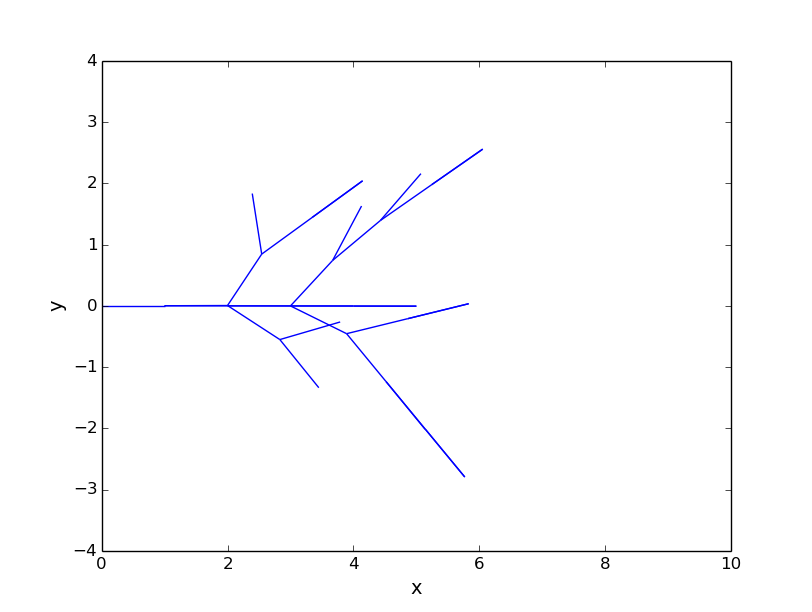
\includegraphics[scale=.5]{images/2D_partonshower.png}
\caption{2D simulation of the spliting of a single parton, here the colour fades as the energy decreases}
\end{figure}

The 3D simulation of the parton shower is essentially the same as for python code with few changes, in which now we have two rotation angles, $\theta$ and also $\phi$ which is the azimuthal angle which is uniformly distributed in the interval [0,2$\pi$]. To simulate the rotation in three dimensions, the function \verb $normv(u)$ and function \verb !rotation(v,angle)!, the former returns the axis of the rotation, the function input and the vector [1,1,1] from a plane, from which we find a vector that is orthogonal to this plane, and the later is matrix of rotation, it takes the angle rotation and the axis of rotation as inputs. 

Also here z (the energy fraction) now is lies the interval[0,1] and the stability limit is 0.05. The digram in figure 4 shows the 3D simulation of single parton splitting.
 
 \begin{figure}[H]
\centering
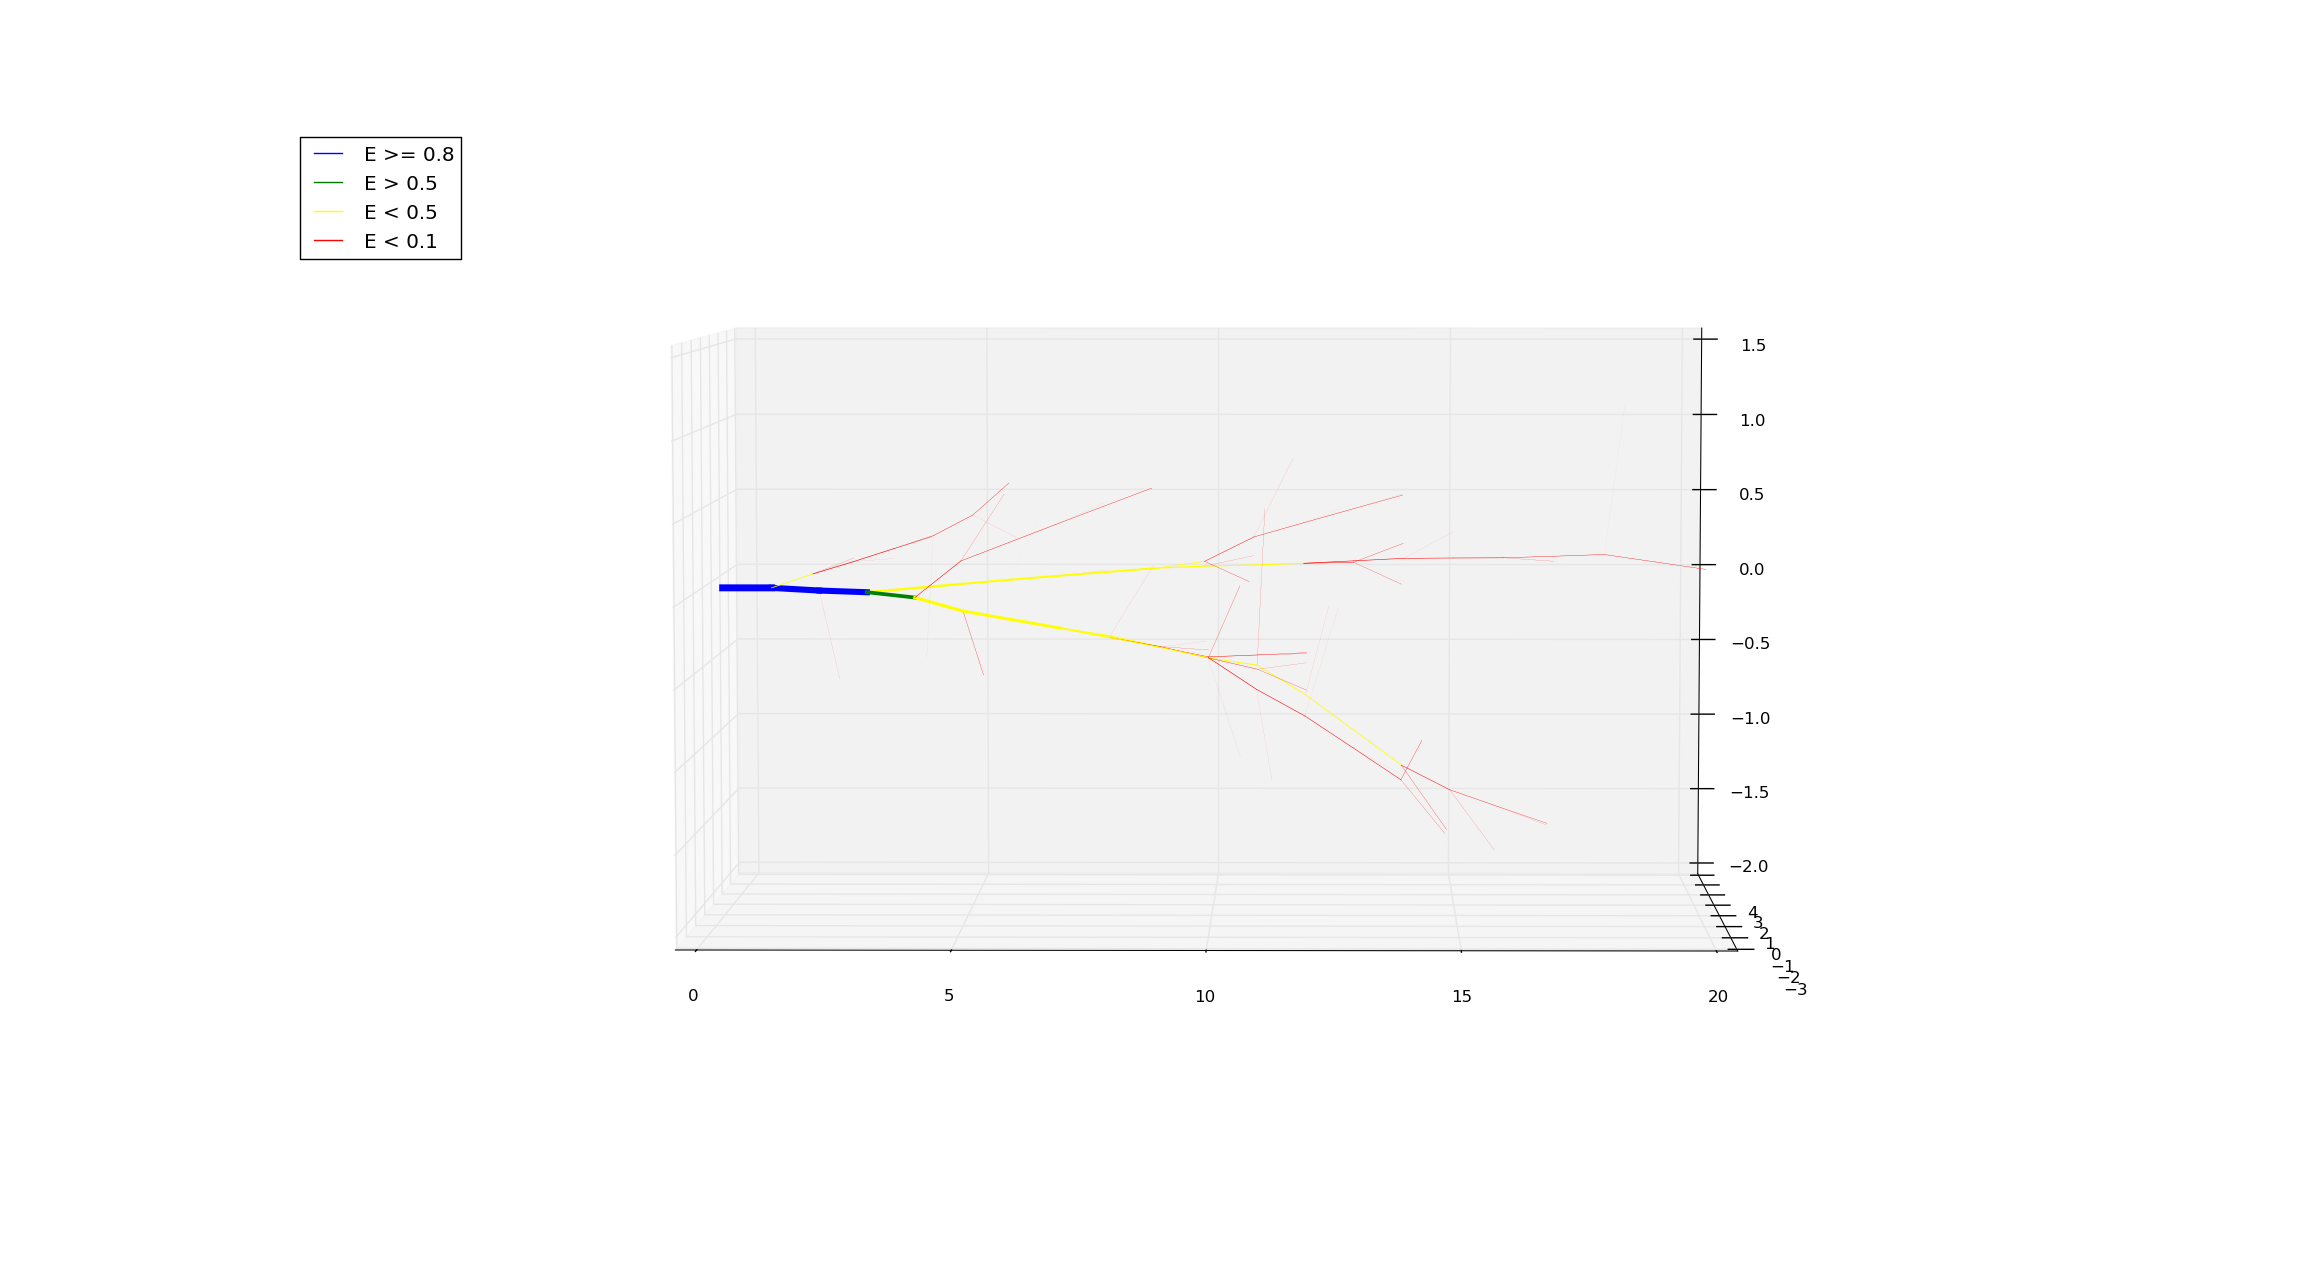
\includegraphics[scale=.3]{images/3D_partonshower.png}
\caption{3D simulation of the spliting of a single parton}
\end{figure}
   
      
  
\end{document}